% Created by tikzDevice version 0.12.3.1 on 2021-09-17 14:13:18
% !TEX encoding = UTF-8 Unicode
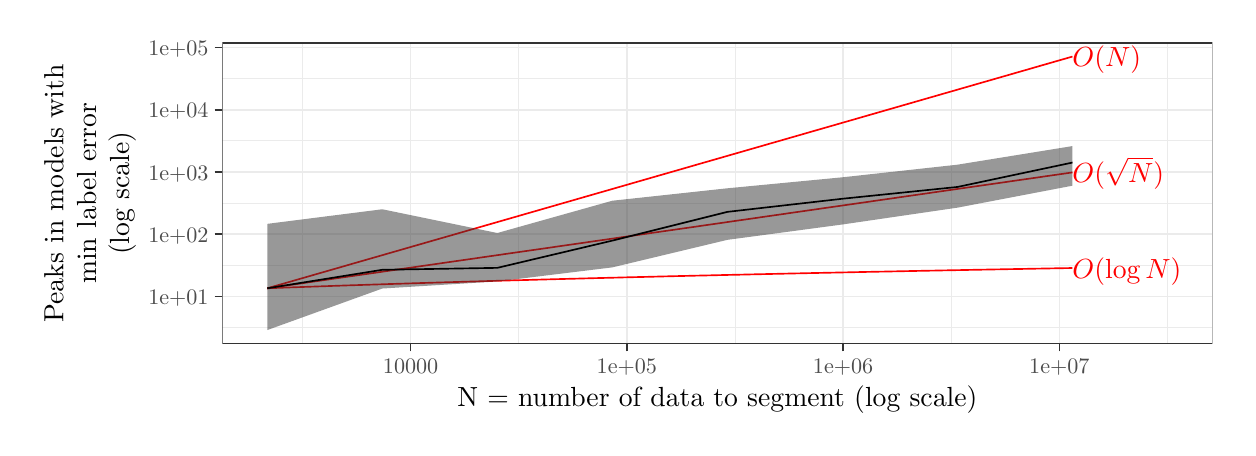
\begin{tikzpicture}[x=1pt,y=1pt]
\definecolor{fillColor}{RGB}{255,255,255}
\path[use as bounding box,fill=fillColor,fill opacity=0.00] (0,0) rectangle (433.62,144.54);
\begin{scope}
\path[clip] (  0.00,  0.00) rectangle (433.62,144.54);
\definecolor{drawColor}{RGB}{255,255,255}
\definecolor{fillColor}{RGB}{255,255,255}

\path[draw=drawColor,line width= 0.6pt,line join=round,line cap=round,fill=fillColor] (  0.00,  0.00) rectangle (433.62,144.54);
\end{scope}
\begin{scope}
\path[clip] ( 70.31, 30.33) rectangle (428.12,139.04);
\definecolor{fillColor}{RGB}{255,255,255}

\path[fill=fillColor] ( 70.31, 30.33) rectangle (428.12,139.04);
\definecolor{drawColor}{gray}{0.92}

\path[draw=drawColor,line width= 0.3pt,line join=round] ( 70.31, 36.20) --
	(428.12, 36.20);

\path[draw=drawColor,line width= 0.3pt,line join=round] ( 70.31, 58.68) --
	(428.12, 58.68);

\path[draw=drawColor,line width= 0.3pt,line join=round] ( 70.31, 81.17) --
	(428.12, 81.17);

\path[draw=drawColor,line width= 0.3pt,line join=round] ( 70.31,103.65) --
	(428.12,103.65);

\path[draw=drawColor,line width= 0.3pt,line join=round] ( 70.31,126.14) --
	(428.12,126.14);

\path[draw=drawColor,line width= 0.3pt,line join=round] ( 99.31, 30.33) --
	( 99.31,139.04);

\path[draw=drawColor,line width= 0.3pt,line join=round] (177.44, 30.33) --
	(177.44,139.04);

\path[draw=drawColor,line width= 0.3pt,line join=round] (255.58, 30.33) --
	(255.58,139.04);

\path[draw=drawColor,line width= 0.3pt,line join=round] (333.72, 30.33) --
	(333.72,139.04);

\path[draw=drawColor,line width= 0.3pt,line join=round] (411.86, 30.33) --
	(411.86,139.04);

\path[draw=drawColor,line width= 0.6pt,line join=round] ( 70.31, 47.44) --
	(428.12, 47.44);

\path[draw=drawColor,line width= 0.6pt,line join=round] ( 70.31, 69.93) --
	(428.12, 69.93);

\path[draw=drawColor,line width= 0.6pt,line join=round] ( 70.31, 92.41) --
	(428.12, 92.41);

\path[draw=drawColor,line width= 0.6pt,line join=round] ( 70.31,114.90) --
	(428.12,114.90);

\path[draw=drawColor,line width= 0.6pt,line join=round] ( 70.31,137.38) --
	(428.12,137.38);

\path[draw=drawColor,line width= 0.6pt,line join=round] (138.38, 30.33) --
	(138.38,139.04);

\path[draw=drawColor,line width= 0.6pt,line join=round] (216.51, 30.33) --
	(216.51,139.04);

\path[draw=drawColor,line width= 0.6pt,line join=round] (294.65, 30.33) --
	(294.65,139.04);

\path[draw=drawColor,line width= 0.6pt,line join=round] (372.79, 30.33) --
	(372.79,139.04);
\definecolor{drawColor}{RGB}{255,0,0}

\path[draw=drawColor,line width= 0.6pt,line join=round] ( 86.58, 50.37) --
	( 89.51, 50.48) --
	( 92.45, 50.59) --
	( 95.39, 50.70) --
	( 98.33, 50.80) --
	(101.27, 50.91) --
	(104.21, 51.01) --
	(107.15, 51.11) --
	(110.09, 51.22) --
	(113.03, 51.32) --
	(115.96, 51.42) --
	(118.90, 51.51) --
	(121.84, 51.61) --
	(124.78, 51.71) --
	(127.72, 51.80) --
	(130.66, 51.90) --
	(133.60, 51.99) --
	(136.54, 52.08) --
	(139.48, 52.18) --
	(142.42, 52.27) --
	(145.35, 52.36) --
	(148.29, 52.45) --
	(151.23, 52.54) --
	(154.17, 52.62) --
	(157.11, 52.71) --
	(160.05, 52.80) --
	(162.99, 52.88) --
	(165.93, 52.97) --
	(168.87, 53.05) --
	(171.80, 53.13) --
	(174.74, 53.22) --
	(177.68, 53.30) --
	(180.62, 53.38) --
	(183.56, 53.46) --
	(186.50, 53.54) --
	(189.44, 53.62) --
	(192.38, 53.70) --
	(195.32, 53.78) --
	(198.25, 53.85) --
	(201.19, 53.93) --
	(204.13, 54.01) --
	(207.07, 54.08) --
	(210.01, 54.16) --
	(212.95, 54.23) --
	(215.89, 54.31) --
	(218.83, 54.38) --
	(221.77, 54.45) --
	(224.71, 54.52) --
	(227.64, 54.60) --
	(230.58, 54.67) --
	(233.52, 54.74) --
	(236.46, 54.81) --
	(239.40, 54.88) --
	(242.34, 54.95) --
	(245.28, 55.01) --
	(248.22, 55.08) --
	(251.16, 55.15) --
	(254.09, 55.22) --
	(257.03, 55.28) --
	(259.97, 55.35) --
	(262.91, 55.42) --
	(265.85, 55.48) --
	(268.79, 55.55) --
	(271.73, 55.61) --
	(274.67, 55.68) --
	(277.61, 55.74) --
	(280.55, 55.80) --
	(283.48, 55.87) --
	(286.42, 55.93) --
	(289.36, 55.99) --
	(292.30, 56.05) --
	(295.24, 56.11) --
	(298.18, 56.17) --
	(301.12, 56.24) --
	(304.06, 56.30) --
	(307.00, 56.36) --
	(309.93, 56.41) --
	(312.87, 56.47) --
	(315.81, 56.53) --
	(318.75, 56.59) --
	(321.69, 56.65) --
	(324.63, 56.71) --
	(327.57, 56.76) --
	(330.51, 56.82) --
	(333.45, 56.88) --
	(336.38, 56.93) --
	(339.32, 56.99) --
	(342.26, 57.05) --
	(345.20, 57.10) --
	(348.14, 57.16) --
	(351.08, 57.21) --
	(354.02, 57.27) --
	(356.96, 57.32) --
	(359.90, 57.37) --
	(362.84, 57.43) --
	(365.77, 57.48) --
	(368.71, 57.53) --
	(371.65, 57.59) --
	(374.59, 57.64) --
	(377.53, 57.69);

\path[draw=drawColor,line width= 0.6pt,line join=round] ( 86.58, 50.37) --
	( 89.51, 50.80) --
	( 92.45, 51.22) --
	( 95.39, 51.64) --
	( 98.33, 52.06) --
	(101.27, 52.49) --
	(104.21, 52.91) --
	(107.15, 53.33) --
	(110.09, 53.76) --
	(113.03, 54.18) --
	(115.96, 54.60) --
	(118.90, 55.02) --
	(121.84, 55.45) --
	(124.78, 55.87) --
	(127.72, 56.29) --
	(130.66, 56.72) --
	(133.60, 57.14) --
	(136.54, 57.56) --
	(139.48, 57.98) --
	(142.42, 58.41) --
	(145.35, 58.83) --
	(148.29, 59.25) --
	(151.23, 59.68) --
	(154.17, 60.10) --
	(157.11, 60.52) --
	(160.05, 60.94) --
	(162.99, 61.37) --
	(165.93, 61.79) --
	(168.87, 62.21) --
	(171.80, 62.64) --
	(174.74, 63.06) --
	(177.68, 63.48) --
	(180.62, 63.90) --
	(183.56, 64.33) --
	(186.50, 64.75) --
	(189.44, 65.17) --
	(192.38, 65.60) --
	(195.32, 66.02) --
	(198.25, 66.44) --
	(201.19, 66.86) --
	(204.13, 67.29) --
	(207.07, 67.71) --
	(210.01, 68.13) --
	(212.95, 68.56) --
	(215.89, 68.98) --
	(218.83, 69.40) --
	(221.77, 69.82) --
	(224.71, 70.25) --
	(227.64, 70.67) --
	(230.58, 71.09) --
	(233.52, 71.52) --
	(236.46, 71.94) --
	(239.40, 72.36) --
	(242.34, 72.78) --
	(245.28, 73.21) --
	(248.22, 73.63) --
	(251.16, 74.05) --
	(254.09, 74.48) --
	(257.03, 74.90) --
	(259.97, 75.32) --
	(262.91, 75.74) --
	(265.85, 76.17) --
	(268.79, 76.59) --
	(271.73, 77.01) --
	(274.67, 77.44) --
	(277.61, 77.86) --
	(280.55, 78.28) --
	(283.48, 78.70) --
	(286.42, 79.13) --
	(289.36, 79.55) --
	(292.30, 79.97) --
	(295.24, 80.40) --
	(298.18, 80.82) --
	(301.12, 81.24) --
	(304.06, 81.66) --
	(307.00, 82.09) --
	(309.93, 82.51) --
	(312.87, 82.93) --
	(315.81, 83.36) --
	(318.75, 83.78) --
	(321.69, 84.20) --
	(324.63, 84.62) --
	(327.57, 85.05) --
	(330.51, 85.47) --
	(333.45, 85.89) --
	(336.38, 86.32) --
	(339.32, 86.74) --
	(342.26, 87.16) --
	(345.20, 87.58) --
	(348.14, 88.01) --
	(351.08, 88.43) --
	(354.02, 88.85) --
	(356.96, 89.28) --
	(359.90, 89.70) --
	(362.84, 90.12) --
	(365.77, 90.54) --
	(368.71, 90.97) --
	(371.65, 91.39) --
	(374.59, 91.81) --
	(377.53, 92.24);

\path[draw=drawColor,line width= 0.6pt,line join=round] ( 86.58, 50.37) --
	( 89.51, 51.22) --
	( 92.45, 52.06) --
	( 95.39, 52.91) --
	( 98.33, 53.76) --
	(101.27, 54.60) --
	(104.21, 55.45) --
	(107.15, 56.29) --
	(110.09, 57.14) --
	(113.03, 57.98) --
	(115.96, 58.83) --
	(118.90, 59.68) --
	(121.84, 60.52) --
	(124.78, 61.37) --
	(127.72, 62.21) --
	(130.66, 63.06) --
	(133.60, 63.90) --
	(136.54, 64.75) --
	(139.48, 65.60) --
	(142.42, 66.44) --
	(145.35, 67.29) --
	(148.29, 68.13) --
	(151.23, 68.98) --
	(154.17, 69.82) --
	(157.11, 70.67) --
	(160.05, 71.52) --
	(162.99, 72.36) --
	(165.93, 73.21) --
	(168.87, 74.05) --
	(171.80, 74.90) --
	(174.74, 75.74) --
	(177.68, 76.59) --
	(180.62, 77.44) --
	(183.56, 78.28) --
	(186.50, 79.13) --
	(189.44, 79.97) --
	(192.38, 80.82) --
	(195.32, 81.66) --
	(198.25, 82.51) --
	(201.19, 83.36) --
	(204.13, 84.20) --
	(207.07, 85.05) --
	(210.01, 85.89) --
	(212.95, 86.74) --
	(215.89, 87.58) --
	(218.83, 88.43) --
	(221.77, 89.28) --
	(224.71, 90.12) --
	(227.64, 90.97) --
	(230.58, 91.81) --
	(233.52, 92.66) --
	(236.46, 93.50) --
	(239.40, 94.35) --
	(242.34, 95.20) --
	(245.28, 96.04) --
	(248.22, 96.89) --
	(251.16, 97.73) --
	(254.09, 98.58) --
	(257.03, 99.42) --
	(259.97,100.27) --
	(262.91,101.12) --
	(265.85,101.96) --
	(268.79,102.81) --
	(271.73,103.65) --
	(274.67,104.50) --
	(277.61,105.34) --
	(280.55,106.19) --
	(283.48,107.04) --
	(286.42,107.88) --
	(289.36,108.73) --
	(292.30,109.57) --
	(295.24,110.42) --
	(298.18,111.26) --
	(301.12,112.11) --
	(304.06,112.96) --
	(307.00,113.80) --
	(309.93,114.65) --
	(312.87,115.49) --
	(315.81,116.34) --
	(318.75,117.18) --
	(321.69,118.03) --
	(324.63,118.88) --
	(327.57,119.72) --
	(330.51,120.57) --
	(333.45,121.41) --
	(336.38,122.26) --
	(339.32,123.10) --
	(342.26,123.95) --
	(345.20,124.80) --
	(348.14,125.64) --
	(351.08,126.49) --
	(354.02,127.33) --
	(356.96,128.18) --
	(359.90,129.02) --
	(362.84,129.87) --
	(365.77,130.72) --
	(368.71,131.56) --
	(371.65,132.41) --
	(374.59,133.25) --
	(377.53,134.10);

\node[text=drawColor,anchor=base west,inner sep=0pt, outer sep=0pt, scale=  1.00] at (377.53,130.39) {$O(N)$};

\node[text=drawColor,anchor=base west,inner sep=0pt, outer sep=0pt, scale=  1.00] at (377.53, 53.98) {$O(\log N)$};

\node[text=drawColor,anchor=base west,inner sep=0pt, outer sep=0pt, scale=  1.00] at (377.53, 88.53) {$O(\sqrt N)$};
\definecolor{fillColor}{RGB}{51,51,51}

\path[fill=fillColor,fill opacity=0.50] ( 86.58, 73.65) --
	(128.14, 78.92) --
	(169.71, 70.34) --
	(211.27, 82.01) --
	(252.84, 86.50) --
	(294.40, 90.47) --
	(335.97, 95.03) --
	(377.53,101.75) --
	(377.53, 87.44) --
	(335.97, 79.50) --
	(294.40, 73.42) --
	(252.84, 67.87) --
	(211.27, 57.92) --
	(169.71, 52.84) --
	(128.14, 50.28) --
	( 86.58, 35.27) --
	cycle;

\path[] ( 86.58, 73.65) --
	(128.14, 78.92) --
	(169.71, 70.34) --
	(211.27, 82.01) --
	(252.84, 86.50) --
	(294.40, 90.47) --
	(335.97, 95.03) --
	(377.53,101.75);

\path[] (377.53, 87.44) --
	(335.97, 79.50) --
	(294.40, 73.42) --
	(252.84, 67.87) --
	(211.27, 57.92) --
	(169.71, 52.84) --
	(128.14, 50.28) --
	( 86.58, 35.27);
\definecolor{drawColor}{RGB}{0,0,0}

\path[draw=drawColor,line width= 0.6pt,line join=round] ( 86.58, 50.37) --
	(128.14, 57.05) --
	(169.71, 57.75) --
	(211.27, 67.59) --
	(252.84, 77.98) --
	(294.40, 82.72) --
	(335.97, 86.98) --
	(377.53, 95.80);
\definecolor{drawColor}{gray}{0.20}

\path[draw=drawColor,line width= 0.6pt,line join=round,line cap=round] ( 70.31, 30.33) rectangle (428.12,139.04);
\end{scope}
\begin{scope}
\path[clip] (  0.00,  0.00) rectangle (433.62,144.54);
\definecolor{drawColor}{gray}{0.30}

\node[text=drawColor,anchor=base east,inner sep=0pt, outer sep=0pt, scale=  0.80] at ( 65.36, 44.49) {1e+01};

\node[text=drawColor,anchor=base east,inner sep=0pt, outer sep=0pt, scale=  0.80] at ( 65.36, 66.97) {1e+02};

\node[text=drawColor,anchor=base east,inner sep=0pt, outer sep=0pt, scale=  0.80] at ( 65.36, 89.46) {1e+03};

\node[text=drawColor,anchor=base east,inner sep=0pt, outer sep=0pt, scale=  0.80] at ( 65.36,111.94) {1e+04};

\node[text=drawColor,anchor=base east,inner sep=0pt, outer sep=0pt, scale=  0.80] at ( 65.36,134.43) {1e+05};
\end{scope}
\begin{scope}
\path[clip] (  0.00,  0.00) rectangle (433.62,144.54);
\definecolor{drawColor}{gray}{0.20}

\path[draw=drawColor,line width= 0.6pt,line join=round] ( 67.56, 47.44) --
	( 70.31, 47.44);

\path[draw=drawColor,line width= 0.6pt,line join=round] ( 67.56, 69.93) --
	( 70.31, 69.93);

\path[draw=drawColor,line width= 0.6pt,line join=round] ( 67.56, 92.41) --
	( 70.31, 92.41);

\path[draw=drawColor,line width= 0.6pt,line join=round] ( 67.56,114.90) --
	( 70.31,114.90);

\path[draw=drawColor,line width= 0.6pt,line join=round] ( 67.56,137.38) --
	( 70.31,137.38);
\end{scope}
\begin{scope}
\path[clip] (  0.00,  0.00) rectangle (433.62,144.54);
\definecolor{drawColor}{gray}{0.20}

\path[draw=drawColor,line width= 0.6pt,line join=round] (138.38, 27.58) --
	(138.38, 30.33);

\path[draw=drawColor,line width= 0.6pt,line join=round] (216.51, 27.58) --
	(216.51, 30.33);

\path[draw=drawColor,line width= 0.6pt,line join=round] (294.65, 27.58) --
	(294.65, 30.33);

\path[draw=drawColor,line width= 0.6pt,line join=round] (372.79, 27.58) --
	(372.79, 30.33);
\end{scope}
\begin{scope}
\path[clip] (  0.00,  0.00) rectangle (433.62,144.54);
\definecolor{drawColor}{gray}{0.30}

\node[text=drawColor,anchor=base,inner sep=0pt, outer sep=0pt, scale=  0.80] at (138.38, 19.46) {10000};

\node[text=drawColor,anchor=base,inner sep=0pt, outer sep=0pt, scale=  0.80] at (216.51, 19.46) {1e+05};

\node[text=drawColor,anchor=base,inner sep=0pt, outer sep=0pt, scale=  0.80] at (294.65, 19.46) {1e+06};

\node[text=drawColor,anchor=base,inner sep=0pt, outer sep=0pt, scale=  0.80] at (372.79, 19.46) {1e+07};
\end{scope}
\begin{scope}
\path[clip] (  0.00,  0.00) rectangle (433.62,144.54);
\definecolor{drawColor}{RGB}{0,0,0}

\node[text=drawColor,anchor=base,inner sep=0pt, outer sep=0pt, scale=  1.00] at (249.22,  7.62) {N = number of data to segment (log scale)};
\end{scope}
\begin{scope}
\path[clip] (  0.00,  0.00) rectangle (433.62,144.54);
\definecolor{drawColor}{RGB}{0,0,0}

\node[text=drawColor,rotate= 90.00,anchor=base,inner sep=0pt, outer sep=0pt, scale=  1.00] at ( 12.89, 84.68) {Peaks in models with};

\node[text=drawColor,rotate= 90.00,anchor=base,inner sep=0pt, outer sep=0pt, scale=  1.00] at ( 24.77, 84.68) {min label error};

\node[text=drawColor,rotate= 90.00,anchor=base,inner sep=0pt, outer sep=0pt, scale=  1.00] at ( 36.65, 84.68) {(log scale)};
\end{scope}
\end{tikzpicture}
